\documentclass[10pt]{article}
\usepackage[polish]{babel}
\usepackage[utf8]{inputenc}
\usepackage[T1]{fontenc}
\usepackage{graphicx}
\usepackage[export]{adjustbox}
\graphicspath{ {./images/} }
\usepackage{amsmath}
\usepackage{amsfonts}
\usepackage{amssymb}
\usepackage[version=4]{mhchem}
\usepackage{stmaryrd}

\title{PESEL }

\author{}
\date{}


\begin{document}
\maketitle
\begin{center}
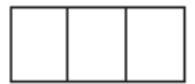
\includegraphics[max width=\textwidth]{2024_11_21_9d761ca624f0efee99a4g-01}
\end{center}

\begin{center}
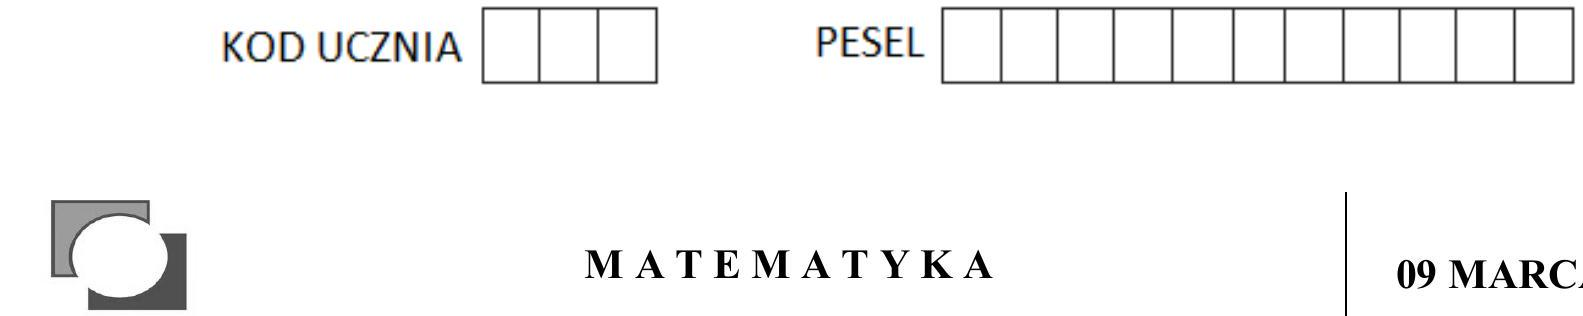
\includegraphics[max width=\textwidth]{2024_11_21_9d761ca624f0efee99a4g-01(2)}
\end{center}

\section*{MATEMATYKA}
09 MARCA 2016\\

\includegraphics[max width=\textwidth, center]{2024_11_21_9d761ca624f0efee99a4g-01(1)}

\section*{Instrukcja dla zdającego}
\begin{enumerate}
  \item Sprawdź, czy arkusz zawiera 14 stron (zadania 1-34). Ewentualny brak zgłoś przewodniczącemu zespołu nadzorującego egzamin.
  \item Rozwiązania zadań i odpowiedzi zamieść w miejscu na to przeznaczonym.
  \item Odpowiedzi do zadań zamkniętych (1-25) przenieś na kartę odpowiedzi, zaznaczając je w części karty przeznaczonej dla zdającego. Zamaluj pola do tego przeznaczone. Błędne zaznaczenie otocz kółkiem i zaznacz właściwe.
  \item Pamiętaj, że pominięcie argumentacji lub istotnych obliczeń w rozwiązaniu zadania otwartego (26-34) może spowodować, że za to rozwiązanie nie otrzymasz pełnej liczby punktów.
  \item Pisz czytelnie i używaj tylko długopisu lub pióra z czarnym tuszem lub atramentem.
  \item Nie używaj korektora, a błędne zapisy wyraźnie przekreśl.
  \item Pamiętaj, że zapisy w brudnopisie nie będą oceniane.
  \item Możesz korzystać z zestawu wzorów matematycznych, cyrkla i linijki oraz kalkulatora prostego.
  \item Na tej stronie oraz na karcie odpowiedzi wpisz swój kod i PESEL (zgodnie z ustaleniami szkolnymi).
  \item Nie wpisuj żadnych znaków w części przeznaczonej dla egzaminatora.
\end{enumerate}

Życzymy powodzenia!

Liczba punktów\\
do uzyskania: \(\mathbf{5 0}\)

\section*{LUBELSKA PRÓBA PRZED MATURĄ 2016 - poziom podstawowy}
\section*{Zadanie 1. (1p)}
Odwrotnością liczby \(8 \sqrt{2}\left(\frac{1}{8}\right)^{-\frac{4}{6}}\) jest liczba\\
A. \(2^{\frac{11}{2}}\)\\
B. \(-2^{\frac{11}{2}}\)\\
C. \(2^{-\frac{11}{2}}\)\\
D. \(-2^{-\frac{11}{2}}\)

\section*{Zadanie 2. (1p)}
Różnica liczby \(x\) i jej kwadratu jest największa dla liczby \(x\) równej\\
A. \(\frac{3}{4}\)\\
B. \(\frac{1}{2}\)\\
C. \(\frac{2}{3}\)\\
D. \(\frac{1}{3}\)

\section*{Zadanie 3. (1p)}
Wśród podanych poniżej nierówności wskaż tę, której zbiorem rozwiązań jest przedział \((-6,8)\)\\
A. \(8<x-2<-6\)\\
B. \(-6<x-2<8\)\\
C. \(-8<x-2<6\)\\
D. \(-8<x+2<6\)

\section*{Zadanie 4. (1p)}
Cenę ksiązki obniżano dwukrotnie, najpierw o 10\%, a po miesiącu jeszcze o 5\%. W wyniku obu obniżek cena książki zmniejszyła się o\\
A. \(14,5 \%\)\\
B. \(14 \%\)\\
C. \(15 \%\)\\
D. \(15,5 \%\)

\section*{Zadanie 5. (1p)}
Liczba o 3 większa od \(\log _{3} 5\) jest równa\\
A. \(\log _{3} 8\)\\
B. \(\log _{3} 135\)\\
C. \(\log _{3} 125\)\\
D. \(\log _{3} 32\)

\section*{Zadanie 6. (1p)}
Na wykresie funkcji liniowej określonej wzorem \(f(x)=(m+2) x+4\) leży punkt \(A=(-2,6)\). Zatem\\
A. \(m=3\)\\
B. \(m=-3\)\\
C. \(m=-4\)\\
D. \(m=4\)

\section*{Zadanie 7. (1p)}
Tangens kąta \(\alpha\) zaznaczonego na rysunku jest równy\\
A. \(\frac{3}{2}\)\\
B. \(-\frac{2}{3}\)\\
C. \(\frac{2}{3}\)\\
D. \(-\frac{3}{2}\)\\
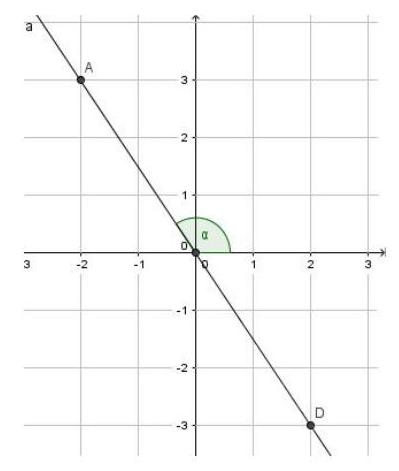
\includegraphics[max width=\textwidth, center]{2024_11_21_9d761ca624f0efee99a4g-02}

\section*{Zadanie 8. (1p)}
Prosta o równaniu \(y=(a-2) x+3\) jest prostopadła do prostej \(y=a x-6\). Zatem\\
A . \(a=-2\)\\
B. \(a=1\)\\
C. \(a=2\)\\
D. \(a=-1\)

\section*{BRUDNOPIS}
\section*{Zadanie 9. (1p)}
Zbiorem wartości funkcji, której wykres przedstawiono na rysunku jest\\
A. \(\langle-2,2)\)\\
B. \((-2,2)\)\\
C. \((-2,2)\)\\
D. \(\langle-2,2\rangle\)\\
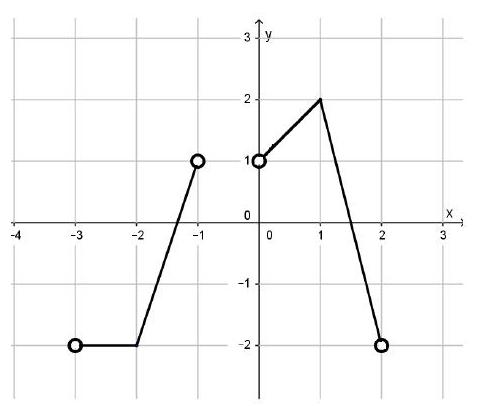
\includegraphics[max width=\textwidth, center]{2024_11_21_9d761ca624f0efee99a4g-04(1)}

\section*{Zadanie 10. (1p)}
Dziedziną funkcji \(f(x)=\frac{x-2}{\sqrt{x-2}}+\frac{2-x}{x}\) jest\\
A. \(x>2\)\\
B. \(x \neq 2\)\\
C. \(x \neq 0\)\\
D. \(x \in R\)

\section*{Zadanie 11. (1p)}
Jeżeli długość przekątnej sześcianu wynosi 3, pole powierzchni całkowitej tego sześcianu jest równe\\
A. \(18 \sqrt{2}\)\\
B. 24\\
C. 18\\
D. \(18 \sqrt{3}\)

Zadanie 12. (1p)\\
Funkcja kwadratowa określona jest wzorem \(f(x)=-x^{2}+2 x+c\). Jeżeli \(f(4)=-2\), to\\
A. \(f(1)=5\)\\
B. \(f(1)=7\)\\
C. \(f(1)=-7\)\\
D. \(f(1)=-5\)

\section*{Zadanie 13. (1p)}
W trapezie równoramiennym (patrz rysunek obok) tangens kąta ostrego \(\alpha\) jest równy\\
A. \(\frac{\sqrt{3}}{3}\)\\
B. \(\frac{\sqrt{2}}{2}\)\\
C. \(\sqrt{3}\)\\
D. \(\sqrt{2}\)\\
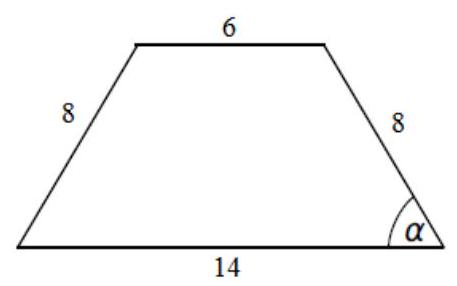
\includegraphics[max width=\textwidth, center]{2024_11_21_9d761ca624f0efee99a4g-04}

Zadanie 14. (1p)\\
Punkty \(A=(-1,-6)\) i \(B=(-7,2)\) są wierzchołkami trójkąta równobocznego \(A B C\). Promień koła opisanego na tym trójkącie jest równy\\
A. \(\frac{10 \sqrt{3}}{6}\)\\
B. \(\frac{5 \sqrt{3}}{3}\)\\
C. \(\frac{10 \sqrt{3}}{3}\)\\
D. \(\frac{5 \sqrt{3}}{6}\)

\section*{Zadanie 15. (1p)}
Dana jest funkcja \(f\) określona wzorem \(f(x)=2^{x}-3\). Wartość funkcji \(g(x)=f(x+1)-1\) dla argumentu \(x=2\) jest równa\\
A. 8\\
B. 6\\
C. 4\\
D. 2

Zadanie 16. (1p)\\
Dla jakiej całkowitej wartości liczby \(\boldsymbol{x}\) spełniona jest nierówność \(\frac{5}{11}<\frac{x}{3}<\frac{25}{33}\) ?\\
A. 1\\
B. 2\\
C. 3\\
D. 4

Zadanie 17. (1p)\\
Miara kąta \(\alpha\) pod jakim przecinają się styczne do okręgu o środku S wynosi\\
A. \(30^{\circ}\)\\
B. \(40^{\circ}\)\\
C. \(60^{\circ}\)\\
D. \(45^{\circ}\)\\
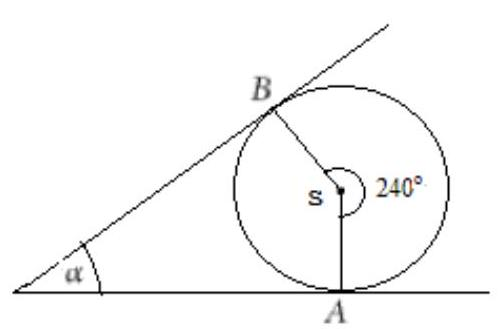
\includegraphics[max width=\textwidth, center]{2024_11_21_9d761ca624f0efee99a4g-06(1)}

Zadanie 18. (1p)\\
Miary kątów czworokąta tworzą ciąg arytmetyczny o pierwszym wyrazie \(45^{\circ}\). Różnica tego ciągu jest równa\\
A . \(40^{\circ}\)\\
B. \(35^{\circ}\)\\
C. \(30^{\circ}\)\\
D. \(25^{\circ}\)

Zadanie 19. (1p)\\
Doświadczenie losowe polega na trzykrotnym rzucie monetą. Prawdopodobieństwo, że dokładnie dwa razy wylosujemy orła wynosi\\
A. \(\frac{3}{6}\)\\
B. \(\frac{3}{7}\)\\
C. \(\frac{3}{9}\)\\
D. \(\frac{3}{8}\)

Zadanie 20. (1p)\\
Dany jest ciąg liczbowy \(\left(a_{n}\right)\), w którym \(a_{1}=x-1, a_{2}=2 x+1, a_{3}=4 x+1\). Dla jakiej wartości liczbowej x dany ciąg jest ciągiem arytmetycznym?\\
A. -2\\
B. 3\\
C. 2\\
D. 4

\section*{Zadanie 21. (1p)}
Ze zbioru liczb naturalnych dwucyfrowych nie większych niż 35 losujemy jedną liczbę. Jakie jest prawdopodobieństwo, że wylosowana liczba będzie podzielna przez 5?\\
A. \(\frac{5}{25}\)\\
B. \(\frac{6}{26}\)\\
C. \(\frac{5}{26}\)\\
D. \(\frac{6}{25}\)

\section*{Zadanie 22. (1p)}
Dla jakich argumentów funkcja \(f(x)=(x+4)(5-x)\) przyjmuje wartości nieujemne?\\
A. \(x \in\langle-4,5\rangle\)\\
B. \(x \in\langle-\infty,-4\rangle \cup\langle 5,+\infty\rangle\)\\
C. \(x \in(-4,5)\)\\
D. \(x \in(-\infty,-4) \cup(5,+\infty)\)

Zadanie 23. (1p)\\
Kąty ABC i ADE są równe oraz \(|A B|=x-3,|B D|=x,|B C|=2\), \(|D E|=8\). Wobec tego x jest równe\\
A. 3\\
B. 3,5\\
C. 4,5\\
D. 4\\
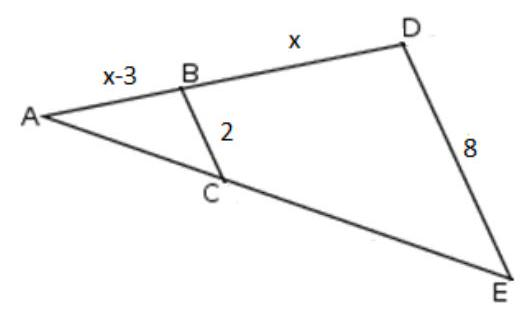
\includegraphics[max width=\textwidth, center]{2024_11_21_9d761ca624f0efee99a4g-06}

\section*{Zadanie 24. (1p)}
Przekątne trapezu ABCD przecinają się w punkcie \(\boldsymbol{K}\) w ten sposób, że \(|\mathrm{AK}|=10,|\mathrm{CK}|=7\), \(|\mathrm{DK}|=5\). Długość odcinka BK jest równa\\
A. 7\\
B. \(3 \frac{1}{2}\)\\
C. 14\\
D. \(7 \frac{1}{7}\)

\section*{LUBELSKA PRÓBA PRZED MATURĄ 2016 - poziom podstawowy}
Zadanie 25. (1p)\\
Podstawą graniastosłupa prostego czworokątnego \(A B C D E F G H\) jest kwadrat \(A B C D\) (zobacz rysunek). Kạt \(A H C\) między przekątnymi sąsiednich ścian bocznych ma \(40^{\circ}\). Kąt \(D B G\) między przekątną podstawy a przekątną ściany bocznej jest równy\\
A. \(70^{\circ}\)\\
B. \(65^{\circ}\)\\
C. \(60^{\circ}\)\\
D. \(55^{\circ}\)\\
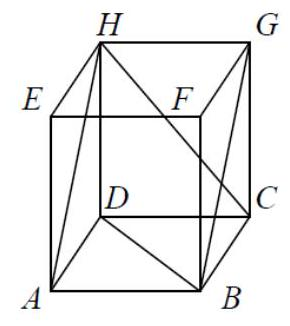
\includegraphics[max width=\textwidth, center]{2024_11_21_9d761ca624f0efee99a4g-07}

\section*{BRUDNOPIS}
\section*{LUBELSKA PRÓBA PRZED MATURĄ 2016 - poziom podstawowy}
\section*{ZADANIA OTWARTE (zmień dane)}
Rozwiązania zadań o numerach od 26 do 34 należy zapisać \(w\) wyznaczonych miejscach pod treścia zadania (pamiętaj o udzieleniu odpowiedzi)

\section*{Zadanie 26. (2p)}
Funkcja kwadratowa \(f\), której miejscami zerowymi są liczby - 5 i 7, dla argumentu 1 przyjmuje wartość -3 . Uzasadnij, że wykres funkcji \(f\) ma dwa punkty wspólne z prostą \(y=-2\).

Odpowiedź:

\section*{Zadanie 27. (2p)}
Rozwiąż nierówność kwadratową \((2 x+1)^{2} \leq 4\).\\

\includegraphics[max width=\textwidth, center]{2024_11_21_9d761ca624f0efee99a4g-08}

Odpowiedź:

\section*{Zadanie 28. (2p)}
W trójkącie prostokątnym, w którym przyprostokątne mają długości 1 i 3, jeden z kątów ostrych ma miarę \(\alpha\). Oblicz wartość wyrażenia \(\sin \alpha+\cos \alpha\).\\

\includegraphics[max width=\textwidth, center]{2024_11_21_9d761ca624f0efee99a4g-08(1)}

Odpowiedź:

\section*{LUBELSKA PRÓBA PRZED MATURĄ 2016 - poziom podstawowy}
\section*{Zadanie 29. (2p)}
Wykres funkcji kwadratowej \(f\) danej wzorem \(f(x)=x^{2}+3 x-4\) przecięto prostymi o równaniach \(x=-1\) oraz \(x=2\). Oblicz odległość między punktami przecięcia tych prostych z wykresem funkcji \(f\).

Odpowiedź:

\section*{Zadanie 30. (2p)}
Uzasadnij, że nierówność \(a^{2}+b^{2} \geq 2 a b-1\) jest prawdziwa dla dowolnych liczb rzeczywistych \(a\) i \(b\).\\

\includegraphics[max width=\textwidth, center]{2024_11_21_9d761ca624f0efee99a4g-09(1)}

\section*{Zadanie 31. (2p)}
Oblicz pole trójkąta \(A B C\), którego boki zawierają się w prostych o równaniach: \(y=0, y=-\frac{3}{5} x-3\) oraz \(y=\frac{1}{3} x-3\).\\

\includegraphics[max width=\textwidth, center]{2024_11_21_9d761ca624f0efee99a4g-09}

Odpowiedź:

\section*{LUBELSKA PRÓBA PRZED MATURĄ 2016 - poziom podstawowy}
\section*{Zadanie 32. (4p)}
Tworząca stożka o kącie rozwarcia \(\alpha\) ma długość 6 . Pole powierzchni całkowitej tego stożka jest równe \(27 \pi\). Oblicz objętość stożka oraz miarę kąta \(\alpha\).

Odpowiedź:\\
Zadanie 33. (4p)\\
Z pojemnika, w którym znajduje się pięć kul: dwie białe i trzy czerwone, losujemy dwa razy po jednej kuli bez zwracania. Oblicz prawdopodobieństwo, że wylosujemy co najmniej jedną kulę czerwoną. Wynik przedstaw w postaci ułamka nieskracalnego.

Odpowiedź:

\section*{Zadanie 34. (5p)}
W roku 2015 na uroczystości urodzinowej ktoś zapytał jubilata, które urodziny obchodzi. Jubilat odpowiedział: jeżeli mój wiek sprzed 27 lat pomnożysz przez mój wiek za 15 lat, to otrzymasz rok mojego urodzenia. Oblicz, ile lat ma ten jubilat.

Odpowiedź:

\section*{BRUDNOPIS}
\section*{BRUDNOPIS}
\section*{BRUDNOPIS}
KARTA ODPOWIEDZI

KOD UCZNIA \(\qquad\)\\
Wypełnia piszacy

\begin{center}
\begin{tabular}{|c|c|c|c|c|}
\hline
\begin{tabular}{c}
Nr \\
zadmia \\
\end{tabular} & A & B & C & D \\
\hline
1. & \(\square\) & \(\square\) & \(\square\) & \(\square\) \\
\hline
2. & \(\square\) & \(\square\) & \(\square\) & \(\square\) \\
\hline
3. & \(\square\) & \(\square\) & \(\square\) & \(\square\) \\
\hline
4. & \(\square\) & \(\square\) & \(\square\) & \(\square\) \\
\hline
5. & \(\square\) & \(\square\) & \(\square\) & \(\square\) \\
\hline
6. & \(\square\) & \(\square\) & \(\square\) & \(\square\) \\
\hline
7. & \(\square\) & \(\square\) & \(\square\) & \(\square\) \\
\hline
8. & \(\square\) & \(\square\) & \(\square\) & \(\square\) \\
\hline
9. & \(\square\) & \(\square\) & \(\square\) & \(\square\) \\
\hline
10. & \(\square\) & \(\square\) & \(\square\) & \(\square\) \\
\hline
11. & \(\square\) & \(\square\) & \(\square\) & \(\square\) \\
\hline
12. & \(\square\) & \(\square\) & \(\square\) & \(\square\) \\
\hline
13. & \(\square\) & \(\square\) & \(\square\) & \(\square\) \\
\hline
14. & \(\square\) & \(\square\) & \(\square\) & \(\square\) \\
\hline
15. & \(\square\) & \(\square\) & \(\square\) & \(\square\) \\
\hline
16. & \(\square\) & \(\square\) & \(\square\) & \(\square\) \\
\hline
17. & \(\square\) & \(\square\) & \(\square\) & \(\square\) \\
\hline
18. & \(\square\) & \(\square\) & \(\square\) & \(\square\) \\
\hline
19. & \(\square\) & \(\square\) & \(\square\) & \(\square\) \\
\hline
20. & \(\square\) & \(\square\) & \(\square\) & \(\square\) \\
\hline
21. & \(\square\) & \(\square\) & \(\square\) & \(\square\) \\
\hline
22. & \(\square\) & \(\square\) & \(\square\) & \(\square\) \\
\hline
23. & \(\square\) & \(\square\) & \(\square\) & \(\square\) \\
\hline
24. & \(\square\) & \(\square\) & \(\square\) & \(\square\) \\
\hline
25. & \(\square\) & \(\square\) & \(\square\) & \(\square\) \\
\hline
\end{tabular}
\end{center}

Razem

PESEL \(\square\)

Wypełnia sprawdzający

\begin{center}
\begin{tabular}{|c|c|c|c|c|}
\hline
\begin{tabular}{c}
Nr \\
zadanis \\
\end{tabular} & X & 0 & 1 & 2 \\
\hline
26. & \(\square\) & \(\square\) & \(\square\) & \(\square\) \\
\hline
27. & \(\square\) & \(\square\) & \(\square\) & \(\square\) \\
\hline
28. & \(\square\) & \(\square\) & \(\square\) & \(\square\) \\
\hline
29. & \(\square\) & \(\square\) & \(\square\) & \(\square\) \\
\hline
30. & \(\square\) & \(\square\) & \(\square\) & \(\square\) \\
\hline
31. & \(\square\) & \(\square\) & \(\square\) & \(\square\) \\
\hline
\end{tabular}
\end{center}

\begin{center}
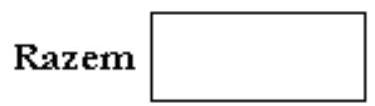
\includegraphics[max width=\textwidth]{2024_11_21_9d761ca624f0efee99a4g-14}
\end{center}

\begin{center}
\begin{tabular}{|c|c|c|c|c|c|c|c|}
\hline
\begin{tabular}{c}
Nin \\
zadmia \\
\end{tabular} & X & 0 & 1 & 2 & 3 & 4 & 5 \\
\hline
32. & \(\square\) & \(\square\) & \(\square\) & \(\square\) & \(\square\) & \(\square\) &  \\
\hline
33. & \(\square\) & \(\square\) & \(\square\) & \(\square\) & \(\square\) & \(\square\) &  \\
\hline
34. & \(\square\) & \(\square\) & \(\square\) & \(\square\) & \(\square\) & \(\square\) & \(\square\) \\
\hline
\end{tabular}
\end{center}

Razem \(\square\)

\begin{center}
\begin{tabular}{|l|l|}
\hline
Suma punktów & Wynik w\% \\
\hline
 &  \\
 &  \\
\hline
\end{tabular}
\end{center}


\end{document}